
\documentclass[8pt,a4paper]{report}
\usepackage[latin1]{inputenc}
\usepackage{amsmath}
\usepackage{amsfonts}
\usepackage{amssymb}
\usepackage{graphicx}
\usepackage{hyperref}
\usepackage{multicol}
\usepackage[margin=0.4in]{geometry}
\usepackage{karnaugh-map}
\usepackage{amsthm}
\usepackage{mathtools}
\usepackage{listings}
\newcommand{\myvec}[1]{\ensuremath{\begin{pmatrix}#1\end{pmatrix}}}
\let\vec\mathbf
\begin{document}

\raggedright{
\includegraphics[scale=0.8]{iith.png}} \hspace{12cm}\raggedleft FWC22084\vspace{8mm}\\ 

\centering \Large \textbf{ASSIGNMENT- MATRICES}
\\ \centering \Large \textbf{CIRCLE} \vspace{15mm}

\begin{multicols}{2}


\raggedright \Large \textbf{Contents} \vspace{2mm}
\begin{itemize}
\raggedright \item Problem \item Solution\item Construction
\end{itemize}\vspace {5mm}
 

\raggedright \Large \textbf{Problem:} \vspace{2mm}
	\\  If a circle passes through the points of intersection of the coordinate axis with the lines $\lambda x-y+1=0$ and $x-2y+3=0$,Find the value of $\lambda$ .\vspace{4mm}
\\\raggedright\Large \textbf{Solution:} \vspace{2mm}
	\\ \raggedright The parametric equation of a circle is \begin{align} \vec{x^{\top}}\vec{x} + 2\vec{u^{\top}}\vec{x} + \textbf{f} = \textbf{0} \end{align} .\vspace{2mm}
	\\ \raggedright The circle passes through the intersection points of the given lines and coordinate axis.\vspace{2mm}
\\\raggedright Equations of given lines and coordinate axis are
                  \begin{align}
			   \myvec{1&-2}\vec{x} = \textbf{-3}
  		         \\  \myvec{\lambda&-1}\vec{x} = \textbf{-1}		
                           \\ \myvec{1&0}\vec{x} = \textbf{0}
			    \\\myvec{0&1}\vec{x} = \textbf{0}
                    \end{align}
   \raggedright Intersection point 1:(p1)
	    \\ \raggedright solving equation 2 and 4 gives us p1
              \begin{align*}
		      \myvec{1&-2\\1&0}\vec{x} = \myvec{-3\\0}
                      \\ \xleftrightarrow[]{R_2 \leftarrow R_2 -R_1 }
			    \myvec{
				    1 & -2 & \vrule & -3
			    \\
			       0 & 2  &\vrule & 3
		    }
		    \\
                     \xleftrightarrow[]{R_1 \leftarrow R_1 +R_2 }
			    \myvec{
				    1 & 0 & \vrule & 0
			    \\
			    0 & 2  &\vrule & 3
		    }
		    \\
                     \xleftrightarrow[]{R_2 \leftarrow \frac{1}{2} R_2 }
			    \myvec{
				    1 & 0 & \vrule & 0
			    \\
			    0 & 1  &\vrule & \frac{3}{2}
		    }
		      \\ \implies \vec{x} = \myvec{0\\\frac{3}{2}}
                  \end{align*}
		   \centering $\vec{p_1} =\vec{x} = k_1\vec{e_2}$\\
     \raggedright Intersection point 2:(p2)
        \\ \raggedright solving equation 2 and 5 gives us p2
                  \begin{align*}
                       \myvec{1&-2\\0&1}\vec{x} = \myvec{-3\\0}
                       \\ \xleftrightarrow[]{R_1 \leftarrow R_1 +2R_2 }
			    \myvec{
				    1 & 0 & \vrule & -3
			    \\
			    0 & 1  &\vrule & 0
		    }
                   \\   \implies \vec{x}= \myvec{-3\\0}
                   \end{align*}
		  \centering   $\vec{p_2} =\vec{x} = k_2\vec{e_1}$\\
      \raggedright  Intersection point 3:(p3)
      \\ \raggedright solving equation 3 and 4 gives us p3
          \begin{align*}
             \myvec{\lambda&-1\\1&0}\vec{x} = \myvec{-1\\0}
                \\ \xleftrightarrow[]{R_1 \leftarrow \frac{1}{\lambda}R_1 }
			    \myvec{
				    1 & -\frac{1}{\lambda} & \vrule & -\frac{1}{\lambda}
			    \\
			    1 & 0  &\vrule & 0
		    }
		    \\
                   \xleftrightarrow[]{R_2 \leftarrow R_2 -R_1 }
			    \myvec{
				    1 & -\frac{1}{\lambda} & \vrule & -\frac{1}{\lambda}
			    \\
			    0 & \frac{1}{\lambda}  &\vrule & \frac{1}{\lambda}
		    }
		    \\
                    \xleftrightarrow[]{R_1 \leftarrow R_2 +R_1 }
			    \myvec{
				    1 & 0 & \vrule & 0
			    \\
			    0 & \frac{1}{\lambda}  &\vrule & \frac{1}{\lambda}
		    }
		    \\
                    \xleftrightarrow[]{R_2 \leftarrow \lambda R_2 }
			    \myvec{
				    1 & 0 & \vrule & 0
			    \\
			    0 & 1  &\vrule & 1
		    }
		  \\   \implies \vec{x} =\myvec{0\\1}
                 \end{align*}
			    \centering $\vec{p_3}=\vec{x}=k_3\vec{e_2}$\\
   \raggedright Intersection point 4:(p4)
 \\ \raggedright solving equation 3 and 5 gives us p4
                 \begin{align*}
                        \myvec{\lambda&-1\\0&1}\vec{x} = \myvec{-1\\0}
                     \\ \xleftrightarrow[]{R_1 \leftarrow R_2 +R_1 }
			    \myvec{
				    \lambda & 0 & \vrule & -1
			    \\
			    0 & 1  &\vrule & 0
		    }
		    \\
                     \xleftrightarrow[]{R_1 \leftarrow \frac{1}{\lambda}R_1 }
			    \myvec{
				    1 & 0 & \vrule & -\frac{1}{\lambda}
			    \\
			    0 & 1  &\vrule & 0
		    }
		    \\  \implies \vec{x} = \myvec{-\frac{1}{\lambda}\\0}
                   \end{align*}
		\centering    $\vec{p_4} =\vec{x}=k_4\vec{e_1}$\\
\raggedright Substituting all the four intersection points in the circle equation gives us the following equations,
              \begin{align}
		      k_1^2 +2k_1\vec{e_2}^{\top}\vec{u} + f = 0
                     \\ k_2^2 +2k_2\vec{e_1}^{\top}\vec{u} + f = 0
                  \\    k_3^2 +2k_3\vec{e_2}^{\top}\vec{u} + f = 0
                    \\  k_4^2 +2k_4\vec{e_1}^{\top}\vec{u} + f = 0   
              \end{align}
 \raggedright To find 'u'and 'f' :\\
                  sloving equations 6, 7 and 8 gives us
                       \begin{align*}
			       \myvec{2k_1\vec{e_2}^{\top}&1\\
			              2k_2\vec{e_1}^{\top}&1\\
				      2k_3\vec{e_2}^{\top}&1}\myvec{u\\f} =\myvec{-k_1^2\\-k_2^2\\-k_3^2}
                         \\ 
			    \myvec{
				    0 & 3 & 1&\vrule & -\frac{9}{4}
			        \\
			            -6 & 0 &1 &\vrule & -9
			        \\
			            0&2&1&\vrule&-1
		                  }
		         \\	
          	           \xleftrightarrow[]{R_1 \leftarrow R_1-R_3 }
			       \myvec{
				       0 & 1 & 0&\vrule & -\frac{5}{4} 
				\\     
				      -6 & 0 & 1&\vrule & -9
			        \\
			               0 & 2&1 &\vrule & -1
		                  }
		         \\
			       \xleftrightarrow[]{R_2 \leftarrow -\frac{R_2}{6} }
			    \myvec{
				     0 & 1 & 0&\vrule & -\frac{5}{4}
			          \\
			             1 & 0  &-\frac{1}{6}&\vrule & \frac{3}{2}
			          \\
			             0&2&1&\vrule&-1
		                  }
		         \\
			       \xleftrightarrow[]{R_1 \leftarrow R_1+R_2 }
			       \myvec{
				       1 & 1 & -\frac{1}{6}&\vrule & \frac{1}{4}
				       \\
				       1 & 0  &-\frac{1}{6}&\vrule & \frac{3}{2}
				       \\
				       0&2&1&\vrule&-1
			         }
			 \\
			       \xleftrightarrow[]{R_2 \leftarrow R_2-R_1 }
			       \myvec{
				       1 & 1 & -\frac{1}{6}&\vrule & -\frac{1}{4}
				       \\
                                             0 & -1  &0&\vrule & \frac{5}{4}
					     \\
					     0&2&1&\vrule&-1
			            }
				    \\
                                \xleftrightarrow[]{R_3 \leftarrow R_3+2R_2 }
			       \myvec{
				       1 & 1 & -\frac{1}{6}&\vrule & \frac{1}{4}
				       \\
				       0 & -1  &0&\vrule & \frac{5}{4}
				       \\
				       0&0&1&\vrule&\frac{3}{2}
				       }
				       \\
                               \xleftrightarrow[]{R_1 \leftarrow R_1+R_2 }
			       \myvec{
				       1 & 0 & -\frac{1}{6}&\vrule & \frac{6}{4}
			              \\
				      0 & 1 &0&\vrule & -\frac{5}{4}
				      \\
				      0&0&1&\vrule&\frac{3}{2}
				      }
				      \\
                             \xleftrightarrow[]{R_1 \leftarrow R_1+\frac{R_3}{6} }
                                 \myvec{
					 1&0&0&\vrule&\frac{7}{4}
					 \\
					 0&1&0&\vrule&-\frac{5}{4}
					 \\
					 0&0&1&\vrule&\frac{3}{2}
					 }
                                          \\
                   \implies \vec{u} =\myvec{\frac{7}{4}\\-\frac{5}{4}}\\
		                f  = \frac{3}{2}
                      \end{align*}
\raggedright To find the value of $\lambda$: \\
\raggedright substituting values of 'u' and 'f' in equation 9 gives us $\lambda$,
                      \begin{align*}
                                       k_4^2 +2k_4\vec{e_1^{\top}}\vec{u} +f =0
                         \end{align*}
              \raggedright Solving the quadratic equation gives us the $k_4$ value as
                    \begin{align*}
			    k_4 =  \frac{-2\vec{e_1^{\top}}\vec{u}\pm\sqrt{(2\vec{e_1^{\top}}\vec{u})^2-4f}}{2}
			    \\ k_4 = \frac{-\frac{7}{2}\pm\sqrt{\frac{25}{4}}}{2}
			    \\ k_4 =  \frac{-\frac{7}{2}\pm\frac{5}{2}}{2}
			    \\ k_4 = -\frac{1}{\lambda} = \frac{-1}{2},-3
                     \end{align*}       	    
		     \raggedright As $\lambda$=$\frac{1}{3}$ is already a point, \\
		            \centering $\lambda$ = 2 \\
\raggedright\Large \textbf{Construction:} \vspace{2mm}
The input parameters for this construction are 
\begin{center}
\begin{tabular}{|c|c|}
	\hline
	\textbf{Symbol}&\textbf{Value}\\
	\hline
	n1&$\
	\begin{pmatrix}
		1 \\
		-2\\
	\end{pmatrix}$%
	\\
	\hline
	n2&$\
	\begin{pmatrix}
		2\\
		-1 \\
	\end{pmatrix}$%
	\\
	\hline
	n3&$\
	\begin{pmatrix}
		0\\
		1\\
	\end{pmatrix}$%
	\\
	\hline
	n4&$\
	\begin{pmatrix}
		1\\
		0\\
	\end{pmatrix}$%
	\\
	\hline
	C1& -3
	\\
	\hline
	C2&-1\\
	\hline
	C&0\\
	\hline
	$\vec{u}$&$\myvec{\frac{7}{4}&-\frac{5}{4}}$% 
	\\
	\hline
	f&$\frac{3}{2}$%
	\\\hline
\end{tabular}
\end{center}
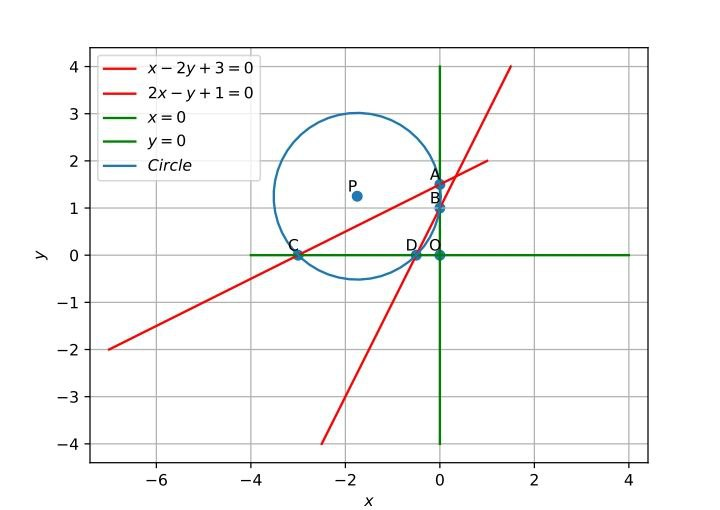
\includegraphics[scale=0.4]{circ.jpg}
The below python code realizes the above construction:	
\centering     https://github.com/reshma0639/FWC-Assignment-1/blob/main/matrices/line.py
\end{multicols}
\end{document}
